\documentclass[handout]{../../../slide}


\title{Unbounded Bivariant K-theory}
\author{Ikhan Choi}
\institute{The University of Tokyo}
\date{Sapporo, September 2024}

% 20 minutes

\begin{document}


\begin{frame}[plain]
\titlepage
\begin{tikzpicture}[remember picture, overlay]
    \node [shift={(2,2)}] at (current page.south west)
        { 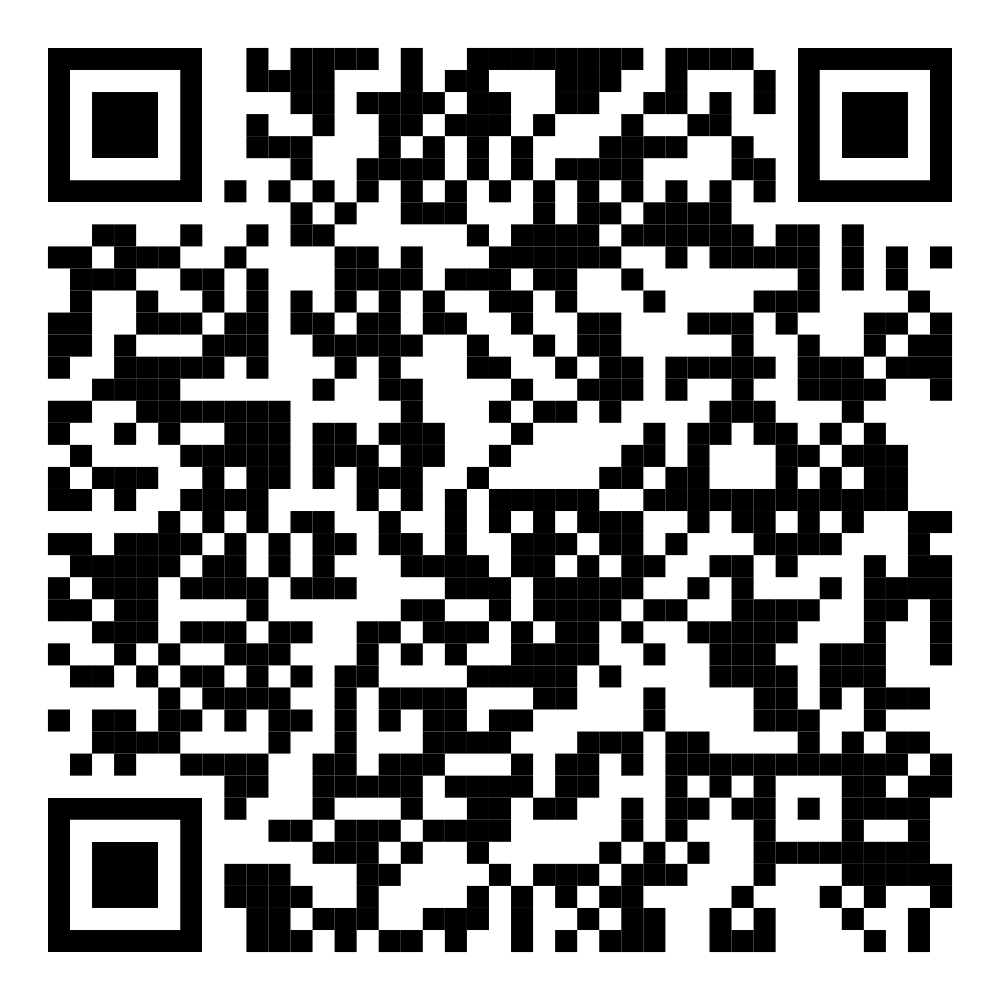
\includegraphics[scale=0.07]{qr} };
\end{tikzpicture}
\end{frame}



\section{Introduction}
\contents


\begin{frame}{Bivariant K-theory}
\begin{defn}[\cite{MR869779}]
The \emph{bivariant K-theory} is a functor $\mathrm{C^*Alg}_{\mathrm{sep}}\to\mathrm{KK}$ which is universal among the homotopy invariant split-exact stable functors to additive categories.
\end{defn}
\pause
\begin{thm}[\cite{MR582160}]
A bivariant K-theory exists.
\end{thm}
\pause
\begin{defn}
The additive category $\mathrm{KK}$ is called the \emph{Kasaprov category}.
The \emph{bivariant K-group} of $A$ and $B$ is the abelian group $KK(A,B)$ of morphisms in the Kasparov category.
\end{defn}
\pause
There are three famous ways to describe the cycles of bivariant K-groups:
\begin{itemize}
\item the Kasparov picture,
\item the Cuntz picture,
\item the Baaj-Julg picture, also called the \emph{unbounded picture}.
\end{itemize}
\end{frame}


\begin{frame}{Unbounded bivariant K-theory}
Pros:
\begin{itemize}
\item We can apply to index theory more directly.
\item We can naturally generalize spectral triples.
\item We can explicitly write down the Kasparov product.
\item We do not need separability or $\sigma$-unitality in principle.
\end{itemize}
\pause
Cons:
\begin{itemize}
\item We do not have a unified definition yet.
\item We cannot characterize the theory in terms of category theory yet.
\item We need to use a lot of unbounded operators on Hilbert modules.
\item We need more complicated and technical conditions depending on references.
\end{itemize}
\end{frame}





\section{Kasparov modules}
\contents


\begin{frame}{Kasparov modules}
\begin{defn}[Right Hilbert bimodules]
A \emph{right Hilbert bimodule} or a \emph{correspondence} over $A$ and $B$ is a right Hilbert module $E$ over $B$ together with a left action of $A$ that is adjointable over $B$.
A right Hilbert bimodule is said to be \emph{countably generated} if it is countably generated as a right Banach module.
A \emph{grading} on a right Hilbert bimodule is an action of $\mathbb{Z}/2\mathbb{Z}$ such that the left and right actions are even.
\end{defn}
\pause
\begin{defn}[Kasparov modules]
A \emph{Kasparov module} is a pair $(E,F)$, where
\begin{itemize}
\item $E$ is a countably generated graded right Hilbert bimodule over $A$ and $B$,
\item $F$ is an odd linear operator on $E$,
\end{itemize}
such that
\begin{enumerate}
\item $F$ is adjointable over $B$,\hfill(adjointability condition)
\item $[F,a]$ is compact for every $a\in A$,\hfill(intertwining condition)
\item $F$ is self-adjoint,\hfill(self-adjoint condition)
\item $(F^2-1)a$ is compact for every $a\in A$.\hfill(Fredholm condition)
\end{enumerate}
\end{defn}
\end{frame}


\begin{frame}{Unbounded Kasparov modules}
\begin{defn}[Regular operators]
A densely defined linear operator $D$ on a right Hilbert module $E$ over $B$ is called \emph{regular} if its graph is a complemented submodule of $E\oplus E$.
\end{defn}
\pause
\begin{defn}[Unbounded Kasparov modules by Baaj-Julg]
An \emph{unbounded Kasparov module} from $A$ to $B$ is a pair $(E,D)$, where
\begin{itemize}
\item $E$ is a countably generated graded right Hilbert bimodule over $A$ and $B$,
\item $D$ is an odd densely-defined linear operator on $E$,
\end{itemize}
such that for some dense $*$-subalgebra $\mathcal{A}\subset A$ we have
\begin{enumerate}
\item $D$ is regular over $B$,\hfill(regularity condition)
\item $\mathcal{A}$ acts on $\operatorname{dom}D$ and $[D,a]$ is adjointable for $a\in\mathcal{A}$,\hfill(Lipschitz condition)
\item $D$ is self-adjoint,\hfill(self-adjoint condition)
\item $(D+i)^{-1}a$ is compact for $a\in\mathcal{A}$.\hfill(compact resolvent condition)
\end{enumerate}
\end{defn}
\pause
If $B=\mathbb{C}$, then an unbounded Kasparov modules is nothing but a spectral triple on $A$ with separable Hilbert space.
\end{frame}




\begin{frame}{Bivariant K-groups}
\begin{defn}
The bivariant K-group $KK(A,B)$ is the abelian group of all homotopy classes of Kasparov modules, where the group structure is given by direct sum.
\end{defn}
\pause
Defining the homotopy equivalence or the direct sum of unbounded Kasparov modules has a domain issue.
It is recently known that there are some solutions modifying the definition of unbounded Kasparov modules for example as in \cite{MR4132745} or \cite{MR4137615}, thereby the existing results dealing with original unbounded Kasparov modules of Baaj-Julg have some difficulties to be applied.
Instead, we can connect unbounded Kasparov modules to bivariant K-theory via an operation called the bounded transform.
\pause
\begin{thm}[\cite{MR715325}]
The bounded transform $(E,D)\mapsto(E,D(1+D^2)^{-\frac12})$ defines
\[\Psi(A,B)\to\mathrm{E}(A,B)\to KK(A,B),\]
and the composition is surjective, where $\mathrm{E}(A,B)$ and $\Psi(A,B)$ are the set of all bounded and unbounded Kasparov modules, respectively.
\end{thm}
\end{frame}





\section{Kasparov product}
\contents


\begin{frame}{Kasparov product}
\begin{defn}[\cite{MR775126}]
A \emph{Kasparov product} of Kasparov modules $(E_1,F_1)$ over $A$ and $B$, and $(E_2,F_2)$ over $B$ and $C$, is a Kasparov module $(E_{12},F_{12})$ over $A$ and $C$ such that
\begin{enumerate}
\item $F_{12}T_{\xi_1}-T_{\overline\xi_1}F_2$ is a compact operator $E_2\to E_{12}$,\hfill(connection condition)
\item $a^*[F_1\otimes1,F_{12}]a$ is positive in the Calkin algebra $Q(E_{12})$,\hfill(positivity condition)
\end{enumerate}
where $E_{12}:=E_1\otimes_BE_2$ and $T_{\xi_1}\xi_2:=\xi_1\otimes\xi_2$.
\end{defn}
\pause
\begin{prop}
There exists a unique Kasparov product of Kasparov modules up to homotopy, hence we have a well-defined bilinear map of abelian groups
\[KK(A,B)\times KK(B,C)\to KK(A,C).\]
Furthermore, the Kasparov product satisfies the conditions for the composition in categories, i.e.~the associativity and the existence of the identity morphisms.
\end{prop}
\end{frame}



\begin{frame}{Unbounded Kasparov product}
Kucerovsky proved the following Connes-Skandalis type theorem for unbounded Kasparove modules.
\pause
\begin{thm}[\cite{MR1435704}]
Let $(E_1,D_1)$, $(E_2,D_2)$ are unbounded Kasparov modules over $A$ and $B$, $B$ and $C$, respectively.
If $(E_{12},D_{12})$ is an unbounded Kasparov module over $A$ and $C$, and if it satisfies
\begin{enumerate}
\item $D_{12}T_{\xi_1}-T_{\overline\xi_1}D_2$ extends to a bounded operator $E_2\to E_{12}$,\hfill(connection condition)
\item $\operatorname{dom}D_{12}\subset\operatorname{dom}(D_1\otimes1)$,\hfill(domain condition)
\item there is $\kappa>0$ such that for every $\xi_{12}\in\operatorname{dom}D_{12}$\hfill(positivity condition)
\[\langle(D_1\otimes1)\xi_{12},D_{12}\xi_{12}\rangle+\langle D_{12}\xi_{12},(D_1\otimes1)\xi_{12}\rangle\ge-\kappa\langle\xi_{12},\xi_{12}\rangle,\]
\end{enumerate}
then it represents a Kasparov product of $(E_1,D_1)$ and $(E_2,D_2)$, via the bounded transform, where $E_{12}:=E_1\otimes_BE_2$ and $T_{\xi_1}\xi_2:=\xi_1\otimes\xi_2$.
\end{thm}
\end{frame}



\begin{frame}{Motivating example}
Let $X$ be a compact Riemannian manifold, and let $A=\mathbb{C}$, $B=C(X)$, and $C=\mathbb{C}$.
\pause
Consider
\begin{itemize}
\item a K-theory class $[(E_1,D_1)]\in KK(\mathbb{C},C(X))$, where
\[E_1:=\Gamma(V),\qquad D_1=0,\qquad V\to X:\text{a Hermitian bundle},\]
\item a K-homology class $[(E_2,D_2)]\in KK(C(X),\mathbb{C})$, where
\[E_2:=L^2(\Omega(X)),\qquad D_2:=d+d^*:\text{the Hodge-Dirac}.\]
\end{itemize}
For $b\in C^\infty(X)$, the commutator $[D_2,b]$ is same as the wedge product with the one-form $db$.
\pause
As a trial for our Kasparov product, consider
\[E_{12}:=E_1\otimes_{C(X)}E_2=L^2(V\otimes\Omega^1(X)),\qquad D_{12}:\stackrel{?}{=}D_1\otimes1+1\otimes D_2.\]
\pause
It is not well-defined since
\[(1\otimes D_2)(\xi_1b\otimes\xi_2)=\overline\xi_1\otimes bD_2\xi_2\ne\overline\xi_1\otimes D_2b\xi_2=(1\otimes D_2)(\xi_1\otimes b\xi_2).\]
\end{frame}



\begin{frame}{Motivating example}
If we introduce a connection $\nabla:\operatorname{dom}\nabla\subset E_1\to E_1\otimes_{C(X)}\Omega^1(X)$ satisfying the Leibniz rule
\[\nabla(\xi_1b)=\nabla(\xi_1)b+\overline\xi_1\otimes[D_2,b],\]
\pause
then by adding a correction term to define a \emph{twisted Dirac operator} $1\otimes_\nabla D_2$ such that
\[(1\otimes_\nabla D_2)(\xi_1\otimes\xi_2):=\overline\xi_1\otimes D_2\xi_2+\nabla(\xi_1)\xi_2,\]
\pause
we can give a well-defined operator on $E_{12}$ as
\begin{align*}
(1\otimes_\nabla D_2)(\xi_1b\otimes\xi_2)&=\overline\xi_1\otimes bD_2\xi_2+\nabla(\xi_1b)\xi_2\\
&=\overline\xi_1\otimes bD_2\xi_2+\nabla(\xi_1)b\xi_2+\overline\xi_1\otimes[D_2,b]\xi_2\\
&=\overline\xi_1\otimes D_2b\xi_2+\nabla(\xi_1)b\xi_2
=(1\otimes_\nabla D_2)(\xi_1\otimes b\xi_2).
\end{align*}
Thus, we suggest
\[D_{12}:=D_1\otimes1+1\otimes_\nabla D_2.\]
\vspace{-8pt}\pause
\begin{itemize}
\item The term $D_{12}T_{\xi_1}-T_{\overline\xi_1}D_2$ is indeed the correction term $\nabla(\xi_1)\xi_2$.
\item If $\nabla$ is Hermitian, then $(E_{12},D_{12})$ is an unbounded Kasparov module satisfying the Kucerovsky condition.
\end{itemize}
\end{frame}



\begin{frame}{Constructive Kasparov product}
We want to consider connections with respect to arbitrary Dirac operators $D_2$.
\begin{defn}
Let $(E_1,D_1)$ and $(E_2,D_2)$ be unbounded Kasparov modules over $A$ and $B$, $B$ and $C$, respectively.
We want to define the \emph{constructive Kasparov product} of $(E_1,D_1)$ and $(E_2,D_2)$, which depends on the choice of $\nabla$ on $E_1$ for $[D_2,-]$, as
\[(E_1\otimes_BE_2,D_1\otimes1+1\otimes_\nabla D_2).\]
\end{defn}
In general, the Dirac operator in constructive Kasparov products may not even be densely defined.
To see it is indeed a representative of the Kasparov product, we have to check all the defining conditions of unbounded Kasparov modules and Kucerovsky's conditions.
There are many case studies on the satisfaction of these conditions, such as the spectral flow of Dirac-Schr\"odinger operators.
See \cite{MR3107519}, \cite{MR3514936} for example.
\end{frame}



\section{Category of spectral triples}
\contents


\begin{frame}{Smooth algebras}
The constructive Kasparov product explicitly retains its spectral geometric data $D_{12}$ before the passage to the bivariant K-group.
It suggests that there would be a differentially refined version of the classical Kasparov product for a category of spectral triples.
\pause
In other words, it would be natural to fix spectral triples on $A$ and $B$ to find another approach which has a non-commutative version of $C^k$ or $W^{k,\infty}$ spaces as domains of $D$ or $\nabla$, requiring that Kucerovsky's conditions automatically follow.
\pause
\begin{defn}[\cite{MR3213549}]
Given an unbounded Kasparov module $(E,D)$ over $A$ and $B$, we define a dense $*$-subalgebra
\[\mathcal{A}^1:=\{a\in A:[D,a]\in\mathcal{L}(E)\},\]
which has a natural operator space structure induced from the embedding
\[\mathcal{A}^1\to\mathcal{L}(M_2(E)):a\mapsto\begin{pmatrix}a&0\\\left[D,a\right]&a\end{pmatrix}.\]
It is a non-commutative analogue of the Sobolev space $W^{1,\infty}$.
\end{defn}
\end{frame}



\begin{frame}[fragile]{Smooth algebras}
\begin{defn}[continued]
We can similarly define $\mathcal{A}^k\subset\mathcal{L}(M_{2^k}(E))$.
We say $(E,D)$ is \emph{smooth} if for each $k$ the algebra $\mathcal{A}^k$ is dense in $A$ and $A$ admits a sequential approximate unit uniformly bounded in $\mathcal{A}^k$.
\end{defn}
\pause
\begin{thm}[\cite{MR3213549}]
Let $A$ and $B$ be endowed with smooth spectral triples.
Let $\Psi_0^\infty(A,B)$ be the set of unitary classes of smooth unbounded Kasparov modules $(E,D,\nabla)$ together with a smooth transverse (we did not define) connection.
Then, the diagram
\[\begin{tikzcd}[sep=small]
\Psi_0^\infty(A,B)\times\Psi_0^\infty(B,C) \rar\dar & \Psi_0^\infty(A,C) \dar\\
KK(A,B)\times KK(B,C) \rar & KK(A,C)
\end{tikzcd}\]
commutes, where horizontal arrows are the (constructive) Kasparov product and vertical arrows are the bounded transforms.
\end{thm}
\end{frame}



\begin{frame}{Correspondences between spectral triples}
\begin{defn}
Let $A$ and $B$ be endowed with smooth spectral triples $(H_{12},D_{12})$ and $(H_2,D_2)$.
Consider the composition law on $\Psi^\infty_0$
\[(E_2,D_2,\nabla^2)\circ(E_1,D_1,\nabla^1):=(E_1\otimes_BE_2,\ D_1\otimes1+1\otimes_{\nabla^1}D_2,\ 1\otimes_{\nabla^1}\nabla^2).\]
A \emph{smooth correspondence} between $A$ and $B$ is a smooth unbounded Kasparov module $(E_1,D_1,\nabla^1)$ over $A$ and $B$ together with a smooth transverse connection such that
\[(H_2,D_2,\mathrm{id})\circ(E_1,D_1,\nabla^1)\sim_u(H_{12},D_{12},\mathrm{id}).\]
\end{defn}
\pause
Smooth correspondences define a symmetric monoidal 2-category, together with a bounded transform functor to the Kasparov category.
One of the ultimate goals is to construct a natural category of spectral triples without assuming some analytic conditions on smoothness.
\end{frame}




\references


\end{document}